%\documentclass[10pt,xcolor={dvipsnames},fleqn]{beamer}
\documentclass[handout,10pt,xcolor={dvipsnames},fleqn]{beamer}
\usepackage{isse}


\usepackage{apalike}
\usepackage[utf8]{inputenc}
\usepackage{pdfpages}
%\usepackage{ngerman}
\usepackage{stmaryrd,amsmath,amssymb}
\usepackage{color}
\usepackage{enumerate}
\usepackage[makeroom]{cancel}
\usepackage{mdframed}
\usepackage{xskak}
\usepackage{fancyvrb}
\usepackage{marvosym}
\setchessboard{
showmover=false}
\usepackage[noend]{algpseudocode}   % package for algorithms
\usepackage{algorithm}
\usepackage{tikz}

\usepackage[absolute,overlay]{textpos}

\usetikzlibrary{trees,calc,shapes,arrows,matrix,shadows,decorations.markings}
\usetikzlibrary{decorations.pathreplacing}
\usetikzlibrary{calc,shapes.callouts,shapes.arrows}
\usetikzlibrary{decorations.text}
\newcommand{\CustomCite}[1]{\color{issegrey} \textbf{#1}}
\tikzset{
   hierNode/.style={main node,text width=1.1em,text centered,inner sep=1pt},
   bStyle/.style={fill=forestgreen!35},
   cStyle/.style={fill=black!35},
   dStyle/.style={fill=thermicred!25},
   optboundaries/.style={
           state,
           rectangle,
           rounded corners,
           draw=black, thick,
           minimum height=4em,
           minimum width=7em,
           inner sep=2pt,
           text centered,
           dashed
           },
  trajectory/.style={issegrey,-},
  emph/.style={isseorange},
  trajectorynode/.style={fill=issegrey},
  hystate/.style={
           state,
           rectangle,
           rounded corners,
           draw=black, very thick,
           minimum height=1em,
           minimum width=2em,
           inner sep=1pt,
           text centered,
           },
 hystatel/.style={
 		   hystate, 
 		   inner sep=3pt
 }
}


\mdfdefinestyle{theoremstyle}{
linecolor=red,linewidth=2pt,
frametitlerule=true,
frametitlebackgroundcolor=gray!20,
innertopmargin=\topskip,
}
\definecolor{LRed}{rgb}{1,.8,.8}
\definecolor{MRed}{rgb}{1,.6,.6}
\definecolor{HRed}{rgb}{1,.2,.2}

\usepackage{listings}
\lstdefinelanguage{mzn}
{
	morekeywords={var,int,solve,not,search,satisfy,new,endif,maximize,params,instantiates,with,bool,in,type,PVS,PVSType,minimize,float,constraint,soft,sum,forall,exists,array,of,include,predicate,then,commit,post,set,function,if,else,repeat,next,ann,break},
	sensitive=false,
	morecomment=[l]{\%},
	morecomment=[s]{/*}{*/},
	morestring=[b]",
}


\definecolor{lightlightgray}{gray}{0.95}
\definecolor{forestgreen}{HTML}{009B55}
\definecolor{thermicred}{rgb}{0.82, 0.1, 0.26}
\lstset
{
	basicstyle=\ttfamily\small,
	commentstyle=\ttfamily\color{thermicred},
	stringstyle=\ttfamily\color{isseorange},
	keywordstyle=\ttfamily\color{blue},
	tabsize=2,
	showstringspaces=false,
	flexiblecolumns=true,
	captionpos=b,	
	backgroundcolor=\color{lightlightgray},
	frame=single,
	 xleftmargin=\parindent,
}

\lstset{language=mzn}
\interfootnotelinepenalty=10000

% ====== custom commands

\newcommand{\prosumer}[1]{\ensuremath{\mathtt{#1}}}
% Soft Constraint Example
\newcommand{\constraintName}[1]{\ensuremath{\mathtt{#1}}}
% Biogas Constraints
\newcommand{\biogas}{biogas}
\newcommand{\biogasShort}{bio}
\newcommand{\gasFull}{\ensuremath{\constraintName{gasFull}_\mathtt{\biogasShort}}}
\newcommand{\ecoSweet}{\ensuremath{\constraintName{ecoSweet}_\mathtt{\biogasShort}}}
\newcommand{\onOff}{\ensuremath{\constraintName{onOff}_\mathtt{\biogasShort}}}
% Thermal Plant Constraints
\newcommand{\thermal}{thermal}
\newcommand{\thermalShort}{therm}
\newcommand{\ecoOpt}{\ensuremath{\constraintName{ecoOpt}_\mathtt{\thermalShort}}}
\newcommand{\inertia}{\ensuremath{\constraintName{inertia}_\mathtt{\thermalShort}}}
\newcommand{\ecoGood}{\ensuremath{\constraintName{ecoGood}_\mathtt{\thermalShort}}}
\newcommand{\hLevelThermal}[1]{$H_#1^\mathtt{\thermalShort}$}
% Electric Vehicle
\newcommand{\ev}{EV}
\newcommand{\limitBatteryUsage}{\ensuremath{\constraintName{limitBU}_\mathtt{\ev}}}
\newcommand{\prefBatteryLevel}{\ensuremath{\constraintName{prefBL}_\mathtt{\ev}}}
\newcommand{\earlyBird}{\ensuremath{\constraintName{earlyBird}_\mathtt{\ev}}}
% Organization
\newcommand{\org}{org}
\newcommand{\minMaxViolation}{\ensuremath{\constraintName{violation}_\mathtt{\org}}}
\newcommand{\hLevelOrg}[1]{$H_#1^\mathtt{\org}$}

\newcommand{\Variable}{X}
\newcommand{\LocalVariable}{\widehat{\Variable}}
\newcommand{\Domain}{D}
\newcommand{\Constraint}{C}
\newcommand{\ConstraintRelationship}{\mathcal{R}}

\newcommand{\valuation}{v}
\newcommand{\constraint}[1]{\mathrm{#1}}

\newcommand{\plantconstraint}[3]{  
\ifx#1b \constraint{best}[#3]
\else \ifx#1g \constraint{good}[#3]
\else \ifx#1a \constraint{acc}[#3]
\else \ifx#1d \constraint{diff}
\else \ifx#1l \constraint{low}[#3]
\else \ifx#1h \constraint{high}[#3]
\else \ifx#1o \constraint{org}[#3]
   \else
   \constraint{#1}_{#2}^{#3} 
   
   
\fi \fi \fi \fi \fi \fi \fi}
\usepackage{stmaryrd}

\providecommand{\smyth}[1]{\prec^{#1}}
\providecommand{\smytheq}[1]{\preceq^{#1}}

\providecommand{\checkfull}{\color{ForestGreen} \checkmark}
\providecommand{\checkhalf}{\color{BurntOrange} (\checkmark)}
\providecommand{\checknot}{\color{BrickRed} $x$}
% booktabs, tables 
\usepackage{booktabs}
\usepackage{tabularx}
\usepackage{longtable}
\usepackage{dcolumn}
\newcolumntype{R}{>{\raggedleft\arraybackslash}X}
\newcolumntype{d}[1]{D{.}{.}{#1} }
\newcolumntype{L}[1]{>{\raggedright\let\newline\\\arraybackslash\hspace{0pt}}m{#1}}


\newcommand{\code}[1]{\normalfont\texttt{\spaceskip=3pt\frenchspacing\def\{{\char123}\def\}{\char125}\def\^{\char94}\def\_{\char95}#1}}
\newcommand{\varit}[1]{{\frenchspacing\ensuremath{\normalfont\textsl{#1}}}}
\newcommand{\macit}[1]{{\frenchspacing\ensuremath{\normalfont\textsf{#1}}}}
\newcommand{\Eta}{\mathrm{H}}
\newcommand{\Mu}{\mathrm{M}}
\newcommand{\Nu}{\mathrm{N}}

\newcommand{\NZ}{\mathbb{N}}
\newcommand{\RZ}{\mathbb{R}}
\newcommand{\RZp}{\RZ_{\geq 0}}
\newcommand{\powerset}{\mathcal{P}}
\newcommand{\limp}{\mathrel{\Rightarrow}}
\newcommand{\compfun}{\mathbin{\circ}}
\newcommand{\isorel}{\mathrel{\cong}}
\newcommand{\restrict}[2]{{#1}\mathnormal{\upharpoonright}{#2}}
\newcommand{\natto}{\mathrel{\dot{\mathnormal{\to}}}}
\let\lbagold\lbag
\let\rbagold\rbag
\def\lbag{\mathopen{\lbagold}}
\def\rbag{\mathclose{\rbagold}}

\DeclareMathOperator{\Minop}{\mathrm{Min}}
\newcommand{\Min}[1]{\Minop^{#1}}
\DeclareMathOperator{\Maxop}{\mathrm{Max}}
\newcommand{\Max}[1]{\Maxop^{#1}}
\DeclareMathOperator{\finsets}{\mathcal{P}_{\mathrm{fin}}}
\DeclareMathOperator{\nefinsets}{\mathcal{P}_{\mathrm{fin}^+}}
%\DeclareMathOperator{\incfinsets}{\mathcal{I}_{\mathrm{fin}}}
\newcommand{\incfinsets}[1]{\mathcal{I}_{\mathrm{fin}}^{#1}}
\newcommand{\lowersubseteq}[1]{\mathrel{\subseteq_{#1}}}
\newcommand{\lowersupseteq}[1]{\mathrel{\supseteq_{#1}}}
\newcommand{\lowersubset}[1]{\mathrel{\subset_{#1}}}
\newcommand{\lowersupset}[1]{\mathrel{\supset_{#1}}}
\newcommand{\uppersubseteq}[1]{\mathrel{\subseteq^{#1}}}
\newcommand{\uppersupseteq}[1]{\mathrel{\supseteq^{#1}}}
\newcommand{\uppersubset}[1]{\mathrel{\subset^{#1}}}
\newcommand{\uppersupset}[1]{\mathrel{\supset^{#1}}}
\newcommand{\lowercup}[1]{\mathbin{\cup_{#1}}}
\newcommand{\uppercup}[1]{\mathbin{\cup^{#1}}}

\DeclareMathOperator{\finmsets}{\mathcal{M}_{\mathrm{fin}}}
\DeclareMathOperator{\nefinmsets}{\mathcal{M}_{\mathrm{fin}^+}}
\newcommand{\mcup}{\mathbin{\mathnormal{\cup}\llap{\text{\fontsize{8pt}{8pt}\selectfont$-$}}}}
\newcommand{\submseteq}{%
\mathrel{\mathchoice%
{\mathnormal{\subseteq}\llap{\text{\raisebox{0.3pt}{\fontsize{8pt}{8pt}\selectfont\rotatebox{90}{$-$}\hspace{1.8pt}}}}}%
{\mathnormal{\subseteq}\llap{\text{\raisebox{0.3pt}{\fontsize{8pt}{8pt}\selectfont\rotatebox{90}{$-$}\hspace{1.8pt}}}}}%
{\mathnormal{\subseteq}\llap{\text{\raisebox{-0.3pt}{\fontsize{5pt}{5pt}\selectfont\rotatebox{90}{$-$}\hspace{1.4pt}}}}}%
{\mathnormal{\subseteq}\llap{\text{\raisebox{-0.3pt}{\fontsize{5pt}{5pt}\selectfont\rotatebox{90}{$-$}\hspace{1.4pt}}}}}%
}}
\newcommand{\supmseteq}{\mathrel{\reflectbox{$\submseteq$}}}
\newcommand{\lowersubmseteq}[1]{\mathrel{\submseteq_{#1}}}
\newcommand{\uppersubmseteq}[1]{\mathrel{\submseteq^{#1}}}
\newcommand{\submset}{%
\mathrel{\mathchoice%
{\mathnormal{\subset}\llap{\text{\raisebox{-0.8pt}{\fontsize{8pt}{8pt}\selectfont\rotatebox{90}{$-$}\hspace{1.8pt}}}}}%
{\mathnormal{\subset}\llap{\text{\raisebox{-0.8pt}{\fontsize{8pt}{8pt}\selectfont\rotatebox{90}{$-$}\hspace{1.8pt}}}}}%
{\mathnormal{\subset}\llap{\text{\raisebox{-0.3pt}{\fontsize{7pt}{7pt}\selectfont\rotatebox{90}{$-$}\hspace{1pt}}}}}%
{\mathnormal{\subset}\llap{\text{\raisebox{-0.3pt}{\fontsize{7pt}{7pt}\selectfont\rotatebox{90}{$-$}\hspace{1pt}}}}}%
}}
\newcommand{\supmset}{\mathrel{\reflectbox{$\submset$}}}
\newcommand{\lowersubmset}[1]{\mathrel{\submset_{#1}}}
\newcommand{\uppersubmset}[1]{\mathrel{\submset^{#1}}}

\DeclareMathOperator{\collapseset}{\mathcal{C}}

\newcommand{\category}[1]{\mathrm{#1}}
\newcommand{\POcat}{\category{PO}}
\newcommand{\uSLcat}{\category{uSL}}
\newcommand{\poMoncat}{\category{poMon}}
\newcommand{\jMoncat}{\category{jMon}}
\newcommand{\mMoncat}{\category{mMon}}
\newcommand{\xMoncat}{{x}\category{Mon}}
\newcommand{\PVScat}{\category{PVS}}
\newcommand{\cSRngcat}{\category{cSRng}}
\newcommand{\DAGcat}{\category{DAG}}

\newcommand{\idfun}[1]{1_{#1}}
\newcommand{\functor}[1]{\mathit{#1}}
\DeclareMathOperator{\POfun}{\functor{PO}}
\DeclareMathOperator{\uSLfun}{\functor{uSL}}
\DeclareMathOperator{\poMonfun}{\functor{poMon}}
\DeclareMathOperator{\jMonfun}{\functor{jMon}}
\DeclareMathOperator{\mMonfun}{\functor{mMon}}
\DeclareMathOperator{\xMonfun}{\text{$x$}\functor{Mon}}
\DeclareMathOperator{\PVSfun}{\functor{PVS}}
\DeclareMathOperator{\cSRngfun}{\functor{cSRng}}
\DeclareMathOperator{\DAGfun}{\functor{DAG}}

\newcommand{\uSLfree}[1]{\uSLfun\langle#1\rangle}
\newcommand{\uSLeta}{\eta^{\uSLcat}}
\newcommand{\uSLetaat}[1]{\uSLeta_{#1}}
\newcommand{\uSLlift}[1]{{#1}^{\sharp_{\uSLcat}}}

\newcommand{\poMonfree}[1]{\poMonfun\langle#1\rangle}
\newcommand{\poMoneta}{\eta^{\poMoncat}}
\newcommand{\poMonetaat}[1]{\poMoneta_{#1}}
\newcommand{\poMonlift}[1]{{#1}^{\sharp_{\poMoncat}}}

\newcommand{\jMonfree}[1]{\jMonfun\langle#1\rangle}
\newcommand{\jMoneta}{\eta^{\jMoncat}}
\newcommand{\jMonetaat}[1]{\jMoneta_{#1}}
\newcommand{\jMonlift}[1]{{#1}^{\sharp_{\jMoncat}}}

\newcommand{\mMonfree}[1]{\mMonfun\langle#1\rangle}
\newcommand{\mMoneta}{\eta^{\mMoncat}}
\newcommand{\mMonetaat}[1]{\mMoneta_{#1}}
\newcommand{\mMonlift}[1]{{#1}^{\sharp_{\mMoncat}}}

\newcommand{\PVSfree}[1]{\PVSfun\langle#1\rangle}
\newcommand{\PVSeta}{\eta^{\PVScat}}
\newcommand{\PVSetaat}[1]{\PVSeta_{#1}}
\newcommand{\PVSlift}[1]{{#1}^{\sharp_{\PVScat}}}

\newcommand{\xMonfree}[1]{\xMonfun\langle#1\rangle}
\newcommand{\xMoneta}{\eta^{\xMoncat}}
\newcommand{\xMonetaat}[1]{\xMoneta_{#1}}
\newcommand{\xMonlift}[1]{{#1}^{\sharp_{\xMoncat}}}

\newcommand{\cSRngfree}[1]{\cSRngfun\langle#1\rangle}
\newcommand{\cSRngeta}{\eta^{\cSRngcat}}
\newcommand{\cSRngetaat}[1]{\cSRngeta_{#1}}
\newcommand{\cSRnglift}[1]{{#1}^{\sharp_{\cSRngcat}}}

\newcommand{\POfree}[1]{\POfun\langle#1\rangle}
\newcommand{\POeta}{\eta^{\POcat}}
\newcommand{\POetaat}[1]{\POeta_{#1}}
\newcommand{\POlift}[1]{{#1}^{\sharp_{\POcat}}}

\newcommand{\mtimes}[1]{\mathbin{\tilde{\cdot}_{#1}}}
\newcommand{\mplus}[1]{\mathbin{\tilde{\cup}_{#1}}}
\newcommand{\ftimes}[1]{\mathbin{\tilde{\mcup}^{#1}}}
\newcommand{\fplus}[1]{\mathbin{\tilde{\cup}_{#1}}}

\DeclareMathOperator{\scope}{\mathrm{sc}}
\DeclareMathOperator{\defdom}{\mathrm{def}}

\newcommand{\reflclos}[1]{\mathrel{(#1)^=}}
\newcommand{\transclos}[2][+]{\mathrel{(#2)^{#1}}}
\newcommand{\refltransclos}[1]{\mathrel{(#1)^*}}

\newcommand{\XPDrel}[2][\pi]{\rightsquigarrow^{#1}_{#2}}
\newcommand{\XPDreleq}[2][\pi]{\rightsquigarrow^{#1, =}_{#2}}
\newcommand{\XPDord}[2][\pi]{<^{#1}_{#2}}
\newcommand{\XPDordeq}[2][\pi]{\geq^{#1}_{#2}}
\newcommand{\XPDleq}[2][\pi]{\leq^{#1}_{#2}}
\newcommand{\XPDgeq}[2][\pi]{\geq^{#1}_{#2}}
\newcommand{\XPDw}[2][\pi]{w^{#1}_{#2}}
\newcommand{\XPDW}[2][\pi]{W^{#1}_{#2}}
\newcommand{\XPDk}[2][\pi]{k^{#1}_{#2}}

\newcommand{\SPDrel}{\XPDrel[\mathrm{SPD}]}
\newcommand{\SPDreleq}{\XPDreleq[\mathrm{SPD}]}
\newcommand{\SPDleq}{\XPDleq[\mathrm{SPD}]}
\newcommand{\SPDgeq}{\XPDgeq[\mathrm{SPD}]}
\newcommand{\SPDord}{\XPDord[\mathrm{SPD}]}
\newcommand{\SPDw}{\XPDw[\mathrm{SPD}]}
\newcommand{\SPDW}{\XPDW[\mathrm{SPD}]}
\newcommand{\DPDrel}{\XPDrel[\mathrm{DPD}]}
\newcommand{\DPDreleq}{\XPDreleq[\mathrm{DPD}]}
\newcommand{\DPDord}{\XPDord[\mathrm{DPD}]}
\newcommand{\DPDw}{\XPDw[\mathrm{DPD}]}
\newcommand{\DPDW}{\XPDW[\mathrm{DPD}]}
\newcommand{\TPDrel}{\XPDrel[\mathrm{TPD}]}
\newcommand{\TPDreleq}{\XPDreleq[\mathrm{TPD}]}
\newcommand{\TPDleq}{\XPDleq[\mathrm{TPD}]}
\newcommand{\TPDgeq}{\XPDgeq[\mathrm{TPD}]}
\newcommand{\TPDord}{\XPDord[\mathrm{TPD}]}
\newcommand{\TPDw}{\XPDw[\mathrm{TPD}]}
\newcommand{\TPDW}{\XPDW[\mathrm{TPD}]}

\DeclareMathSymbol{\UPi}{\mathalpha}{operators}{"05}



\renewcommand{\submseteq}{%
\mathrel{\mathchoice%
{\mathnormal{\subseteq}\llap{\text{\raisebox{0.0pt}{\fontsize{7.5pt}{7.5pt}\selectfont\rotatebox{90}{$-$}\hspace{1.6pt}}}}}%
{\mathnormal{\subseteq}\llap{\text{\raisebox{0.0pt}{\fontsize{7.5pt}{7.5pt}\selectfont\rotatebox{90}{$-$}\hspace{1.6pt}}}}}%
{\mathnormal{\subseteq}\llap{\text{\raisebox{-0.3pt}{\fontsize{7pt}{7pt}\selectfont\rotatebox{90}{$-$}\hspace{1pt}}}}}%
{\mathnormal{\subseteq}\llap{\text{\raisebox{-0.3pt}{\fontsize{7pt}{7pt}\selectfont\rotatebox{90}{$-$}\hspace{1pt}}}}}%
}}


\tikzset{
   main node/.style={circle,fill=black!15,draw,font=\sffamily},
   constraint node/.style={main node, circle, inner sep=2pt,font=\sffamily\small},   
   treestyle/.style={rectangle,fill=black!15,draw,font=\sffamily}
}


\mdtheorem[style=theoremstyle]{definition}{Definition}

\renewcommand{\vec}[1]{\mathbf{#1}}
\newcommand{\tupleOf}[1]{\langle #1 \rangle}
\newcommand{\cemph}[1]{\alert{#1}}
\usepackage{framed}
\usepackage{ifthen}

\usetikzlibrary{decorations.pathmorphing,calc,shadows.blur,shadings}
\usetikzlibrary{mindmap,trees,automata,arrows}
\usepackage{extrabeamercmds}

\newcommand{\hFirst}[1]{{\color{isseorange} #1}}
\newcommand{\hSecond}[1]{{\color{CornflowerBlue} #1}}

\newcounter{mathseed}
\setcounter{mathseed}{3}
\pgfmathsetseed{\arabic{mathseed}} % To have predictable results
% Define a background layer, in which the parchment shape is drawn
\pgfdeclarelayer{background}
\pgfsetlayers{background,main}


% This is the base for the fractal decoration. It takes a random point between the start and end, and
% raises it a random amount, thus transforming a segment into two, connected at that raised point
% This decoration can be applied again to each one of the resulting segments and so on, in a similar
% way of a Koch snowflake.
\pgfdeclaredecoration{irregular fractal line}{init}
{
  \state{init}[width=\pgfdecoratedinputsegmentremainingdistance]
  {
    \pgfpathlineto{\pgfpoint{random*\pgfdecoratedinputsegmentremainingdistance}{(random*\pgfdecorationsegmentamplitude-0.02)*\pgfdecoratedinputsegmentremainingdistance}}
    \pgfpathlineto{\pgfpoint{\pgfdecoratedinputsegmentremainingdistance}{0pt}}
  }
}


% define some styles
\tikzset{
   paper/.style={draw=black!10, blur shadow, every shadow/.style={opacity=1, black}, 
                 lower left=black!10, upper left=black!5, upper right=white, lower right=black!5, fill=none},
   irregular cloudy border/.style={decoration={irregular fractal line, amplitude=0.2},
           decorate,
     },
   irregular spiky border/.style={decoration={irregular fractal line, amplitude=-0.2},
           decorate,
     },
   ragged border/.style={ decoration={random steps, segment length=7mm, amplitude=2mm},
           decorate,
   }
}

\tikzset{
  normal border/.style={orange!30!black!10, decorate, 
     decoration={random steps, segment length=2.5cm, amplitude=.7mm}},
  torn border/.style={orange!30!black!5, decorate, 
     decoration={random steps, segment length=.5cm, amplitude=1.7mm}}}


\def\tornpaper#1{%
\ifthenelse{\isodd{\value{mathseed}}}{%
\tikz{
  \node[inner sep=1em] (A) {#1};  % Draw the text of the node
  \begin{pgfonlayer}{background}  % Draw the shape behind
  \fill[paper] % recursively decorate the bottom border
     \pgfextra{\pgfmathsetseed{\arabic{mathseed}}\addtocounter{mathseed}{1}}%
      {decorate[irregular cloudy border]{decorate{decorate{decorate{decorate[ragged border]{
        (A.north west) -- (A.north east)
      }}}}}}
      -- (A.south east)
     \pgfextra{\pgfmathsetseed{\arabic{mathseed}}}%
      {decorate[irregular spiky border]{decorate{decorate{decorate{decorate[ragged border]{
      -- (A.south west)
      }}}}}}
      -- (A.north west);
  \end{pgfonlayer}}
}{%
\tikz{
  \node[inner sep=1em] (A) {#1};  % Draw the text of the node
  \begin{pgfonlayer}{background}  % Draw the shape behind
  \fill[paper] % recursively decorate the bottom border
     \pgfextra{\pgfmathsetseed{\arabic{mathseed}}\addtocounter{mathseed}{1}}%
      {decorate[irregular spiky border]{decorate{decorate{decorate{decorate[ragged border]{
        (A.north east) -- (A.north west)
      }}}}}}
      -- (A.south west)
     \pgfextra{\pgfmathsetseed{\arabic{mathseed}}}%
      {decorate[irregular cloudy border]{decorate{decorate{decorate{decorate[ragged border]{
      -- (A.south east)
      }}}}}}
      -- (A.north east);
  \end{pgfonlayer}}
}}


% Macro to draw the shape behind the text, when it fits completly in the
% page
\def\parchmentframe#1{
\tikz{
  \node[inner sep=2em] (A) {#1};  % Draw the text of the node
  \begin{pgfonlayer}{background}  % Draw the shape behind
  \fill[normal border] 
        (A.south east) -- (A.south west) -- 
        (A.north west) -- (A.north east) -- cycle;
  \end{pgfonlayer}}}

% Macro to draw the shape, when the text will continue in next page
\def\parchmentframetop#1{
\tikz{
  \node[inner sep=2em] (A) {#1};    % Draw the text of the node
  \begin{pgfonlayer}{background}    
  \fill[normal border]              % Draw the ``complete shape'' behind
        (A.south east) -- (A.south west) -- 
        (A.north west) -- (A.north east) -- cycle;
  \fill[torn border]                % Add the torn lower border
        ($(A.south east)-(0,.2)$) -- ($(A.south west)-(0,.2)$) -- 
        ($(A.south west)+(0,.2)$) -- ($(A.south east)+(0,.2)$) -- cycle;
  \end{pgfonlayer}}}

% Macro to draw the shape, when the text continues from previous page
\def\parchmentframebottom#1{
\tikz{
  \node[inner sep=2em] (A) {#1};   % Draw the text of the node
  \begin{pgfonlayer}{background}   
  \fill[normal border]             % Draw the ``complete shape'' behind
        (A.south east) -- (A.south west) -- 
        (A.north west) -- (A.north east) -- cycle;
  \fill[torn border]               % Add the torn upper border
        ($(A.north east)-(0,.2)$) -- ($(A.north west)-(0,.2)$) -- 
        ($(A.north west)+(0,.2)$) -- ($(A.north east)+(0,.2)$) -- cycle;
  \end{pgfonlayer}}}

% Macro to draw the shape, when both the text continues from previous page
% and it will continue in next page
\def\parchmentframemiddle#1{
\tikz{
  \node[inner sep=2em] (A) {#1};   % Draw the text of the node
  \begin{pgfonlayer}{background}   
  \fill[normal border]             % Draw the ``complete shape'' behind
        (A.south east) -- (A.south west) -- 
        (A.north west) -- (A.north east) -- cycle;
  \fill[torn border]               % Add the torn lower border
        ($(A.south east)-(0,.2)$) -- ($(A.south west)-(0,.2)$) -- 
        ($(A.south west)+(0,.2)$) -- ($(A.south east)+(0,.2)$) -- cycle;
  \fill[torn border]               % Add the torn upper border
        ($(A.north east)-(0,.2)$) -- ($(A.north west)-(0,.2)$) -- 
        ($(A.north west)+(0,.2)$) -- ($(A.north east)+(0,.2)$) -- cycle;
  \end{pgfonlayer}}}

% Define the environment which puts the frame
% In this case, the environment also accepts an argument with an optional
% title (which defaults to ``Example'', which is typeset in a box overlaid
% on the top border
\newenvironment{parchment}[1][Example]{%
  \def\FrameCommand{\parchmentframe}%
  \def\FirstFrameCommand{\parchmentframetop}%
  \def\LastFrameCommand{\parchmentframebottom}%
  \def\MidFrameCommand{\parchmentframemiddle}%
  \vskip\baselineskip
  \MakeFramed {\FrameRestore}
  \noindent\tikz\node[inner sep=1ex, draw=black!20,fill=white, 
          anchor=west, overlay] at (0em, 2em) {\sffamily#1};\par}%
{\endMakeFramed}


\title{MiniBrass: Soft Constraint Programming}
\author{Alexander Schiendorfer et al.}

\date{\today}

\begin{document}
\titleframe

\begin{frame}{Einordnung}
Wo wir letztes Jahr waren \ldots 
\end{frame}


{

\addtobeamertemplate{background canvas}{\transfade[duration=0.001]}{}
%gets rid of bottom navigation bars
\setbeamertemplate{footline}[frame number]{}

%gets rid of bottom navigation symbols
\setbeamertemplate{navigation symbols}{}

%gets rid of footer
%will override 'frame number' instruction above
%comment out to revert to previous/default definitions
\setbeamertemplate{footline}{}

\begin{frame}{Fahrplanerstellungsproblem}
\textbf{Ziel}: Plane Kraftwerke so ein, dass sie die \alert{Last} gemeinsam erfüllen
\tikzset{
    trajectory/.style={issegrey},
    emph/.style={isseorange},
    trajectorynode/.style={issegrey},
    demand/.style={MidnightBlue, thick},
    firstTraj/.style={ForestGreen},
    secTraj/.style={BrickRed}
} 
\begin{figure}
\begin{tikzpicture}[scale=1.0]
    % Draw axes
    \draw [<->,thick] (0,5) node (yaxis) [above] {$P(t)$}
        |- (8.5,0) node (xaxis) [right] {$t$};
        
    \node[overlay,text width=1.9cm, text centered, anchor=south, right] at (7.7,4.5)
    { \small 
    \begin{itemize} 
    \item[] { \color{MidnightBlue} \onslide<2->{\textbf{Demand}} } 
    \item[] { \color{ForestGreen} \onslide<3->{Plant $a$} } 
    \item[] { \color{BrickRed} \onslide<4->{Plant $b$} }  
    \item[] { \color{isseorange} \onslide<5->{\textbf{Supply}} }    
    \end{itemize}
    };        
       
	
%	\node[text width = 1.5cm ,text centered, anchor=west, right] at (2.5, 1)
%	{
%		$\mathbf{+}$
%	};
	
    %\node[text width=2.5cm, text centered, anchor=west, right] at (4,-.5)
    %{
    %		Kraftwerk $\mathsf{b}$
	%}; 
	
	%\node[text width = 1.5cm ,text centered, anchor=west, right] at (6.5, 1)
	%{
	%	$\mathbf{=}$
%	};
	%\node[text width=2.5cm, text centered, anchor=west, right] at (8,-.5)
    %{
    %		Demand
	%};      
    
     % draw second trajectory first graph 
     \onslide<2->{
    \draw[trajectory,demand] (0,3.9) coordinate (d20) -- (1,4.6) coordinate (d21);
    \draw[trajectory,demand] (d21) -- (2,4.4) coordinate (d22);
    \draw[trajectory,demand] (d22) -- (3,4.7) coordinate (d23);
    \draw[trajectory,demand] (d23) -- (4,3.5) coordinate (d24);
    \draw[trajectory,demand] (d24) -- (5,3.5) coordinate (d25);
    \draw[trajectory,demand] (d25) -- (6,3.5) coordinate (d26);
    \draw[trajectory,demand] (d26) -- (7,4.0) coordinate (d27);
    \draw[trajectory,demand] (d27) -- (8,4.5) coordinate (d28);
    
    % now for the circles
    \fill[trajectorynode,demand] (d21) circle (1pt);
    \fill[trajectorynode,demand] (d22) circle (1pt);
    \fill[trajectorynode,demand] (d23) circle (1pt);
    \fill[trajectorynode,demand] (d24) circle (1pt);    
    \fill[trajectorynode,demand] (d25) circle (1pt);
    \fill[trajectorynode,demand] (d26) circle (1pt);
    \fill[trajectorynode,demand] (d27) circle (1pt);
    \fill[trajectorynode,demand] (d28) circle (1pt);
    }
        
    \onslide<3->{
    % now for the first plant   
    \draw[trajectory,firstTraj] (0,1.9) coordinate (p10) -- (1,2.0) coordinate (p11);
    \draw[trajectory,firstTraj] (p11) -- (2,2.4) coordinate (p12);
    \draw[trajectory,firstTraj] (p12) -- (3,2.4) coordinate (p13);
    \draw[trajectory,firstTraj] (p13) -- (4,2.2) coordinate (p14);
    \draw[trajectory,firstTraj] (p14) -- (5,2.4) coordinate (p15);
    \draw[trajectory,firstTraj] (p15) -- (6,2.4) coordinate (p16);
    \draw[trajectory,firstTraj] (p16) -- (7,2.4) coordinate (p17);                   
    \draw[trajectory,firstTraj] (p17) -- (8,2.6) coordinate (p18);
    
    	\onslide<6>{
       \draw[trajectory,firstTraj,very thick] (p11) -- (p12);	
       \node[overlay,align=left,rectangle callout,%
             callout absolute pointer=(p11.west),xshift=-.5cm,yshift=-1.5cm,fill=isseorange!50] at (p12) {
            \scriptsize \textbf{Must} ramp up \\ \scriptsize due to inertia};
       
	}    
    
 	\onslide<8>{
       \draw[trajectory,firstTraj,very thick] (p15) -- (p16);	
       \draw[trajectory,firstTraj,very thick] (p16) -- (p17);
       
          \node[overlay,align=left,rectangle callout,%
             callout absolute pointer=(p16.north),xshift=-.5cm,yshift=0.55cm,fill=isseorange!50] at (p15) {
           \scriptsize  Wait 2 steps for \\ \scriptsize further ramp-up};
	} 
	
    % now for the circles of the first graph
    \fill[trajectorynode,firstTraj] (p11) circle (1pt);
    \fill[trajectorynode,firstTraj] (p12) circle (1pt);
    \fill[trajectorynode,firstTraj] (p13) circle (1pt);
    \fill[trajectorynode,firstTraj] (p14) circle (1pt);    
    \fill[trajectorynode,firstTraj] (p15) circle (1pt);
    \fill[trajectorynode,firstTraj] (p16) circle (1pt);
    \fill[trajectorynode,firstTraj] (p17) circle (1pt);
    \fill[trajectorynode,firstTraj] (p18) circle (1pt);        
    }
    
    \onslide<4->{
    % now for the second plant   
    \draw[trajectory,secTraj] (0,2.0) coordinate (p20) -- (1,2.6) coordinate (p21);
    \draw[trajectory,secTraj] (p21) -- (2,2.0) coordinate (p22);
    \draw[trajectory,secTraj] (p22) -- (3,2.2) coordinate (p23);
    \draw[trajectory,secTraj] (p23) -- (4,1.5) coordinate (p24);
    \draw[trajectory,secTraj] (p24) -- (5,1.4) coordinate (p25);
    \draw[trajectory,secTraj] (p25) -- (6,1.2) coordinate (p26);
    \draw[trajectory,secTraj] (p26) -- (7,1.6) coordinate (p27);                   
    \draw[trajectory,secTraj] (p27) -- (8,1.9) coordinate (p28);
	\onslide<6>{
       \draw[trajectory,secTraj,very thick] (p21) -- (p22);	
       \node[overlay,align=left,rectangle callout,%
             callout absolute pointer=(p21.north),xshift=+1cm,yshift=.5cm,fill=isseorange!50] at (p21) {
            \scriptsize Has to compensate};
	}    
	
	\onslide<7>{
       \draw[trajectory,secTraj,very thick] (p23) -- (p24);	
       \node[overlay,align=left,rectangle callout,%
             callout absolute pointer=(p24.south),xshift=+1cm,yshift=-.8cm,fill=isseorange!50] at (p24) {
             \scriptsize Cannot ramp down further \\ \scriptsize due to inertia};
	}    
    
     % now for the circles of the second graph
    \fill[trajectorynode,secTraj] (p21) circle (1pt);
    \fill[trajectorynode,secTraj] (p22) circle (1pt);
    \fill[trajectorynode,secTraj] (p23) circle (1pt);
    \fill[trajectorynode,secTraj] (p24) circle (1pt);    
    \fill[trajectorynode,secTraj] (p25) circle (1pt);
    \fill[trajectorynode,secTraj] (p26) circle (1pt);
    \fill[trajectorynode,secTraj] (p27) circle (1pt);
    \fill[trajectorynode,secTraj] (p28) circle (1pt);
    }
    
    \onslide<5->{
    % draw joint production first graph 
    \draw[trajectory,emph] (0,3.9) coordinate (s20) -- (1,4.6) coordinate (s21);
    \draw[trajectory,emph] (s21) -- (2,4.4) coordinate (s22);
    \draw[trajectory,emph] (s22) -- (3,4.6) coordinate (s23);
    \draw[trajectory,emph] (s23) -- (4,3.7) coordinate (s24);
    \draw[trajectory,emph] (s24) -- (5,3.8) coordinate (s25);
    \draw[trajectory,emph] (s25) -- (6,3.6) coordinate (s26);
    \draw[trajectory,emph] (s26) -- (7,4.0) coordinate (s27);
    \draw[trajectory,emph] (s27) -- (8,4.5) coordinate (s28);
    
	% now for the circles of the sum
    \fill[trajectorynode,emph] (s21) circle (1pt);
    \fill[trajectorynode,emph] (s22) circle (1pt);
    \fill[trajectorynode,emph] (s23) circle (1pt);
    \fill[trajectorynode,emph] (s24) circle (1pt);    
    \fill[trajectorynode,emph] (s25) circle (1pt);
    \fill[trajectorynode,emph] (s26) circle (1pt);
    \fill[trajectorynode,emph] (s27) circle (1pt);
    \fill[trajectorynode,emph] (s28) circle (1pt);
    }
    
	\node[text centered, anchor=north] at (1,0) { 1 }; \draw[thick] (1,0.05) -- (1,-.05);
	\node[text centered, anchor=north] at (2,0) { 2 }; \draw[thick] (2,0.05) -- (2,-.05);
	\node[text centered, anchor=north] at (3,0) { 3 }; \draw[thick] (3,0.05) -- (3,-.05);	
	\node[text centered, anchor=north] at (4,0) { 4 }; \draw[thick] (4,0.05) -- (4,-.05);
	\node[text centered, anchor=north] at (5,0) { 5 }; \draw[thick] (5,0.05) -- (5,-.05);
	\node[text centered, anchor=north] at (6,0) { 6 }; \draw[thick] (6,0.05) -- (6,-.05);
	\node[text centered, anchor=north] at (7,0) { 7 }; \draw[thick] (7,0.05) -- (7,-.05);	
	\node[text centered, anchor=north] at (8,0) { 8 }; \draw[thick] (8,0.05) -- (8,-.05);
	    

\end{tikzpicture}
\end{figure}  
\end{frame}
}


\begin{frame}{Hierarchisches Energiemanagement}

\begin{figure}
\centering
\begin{tikzpicture}[->,>=stealth',shorten >=1pt,auto,node distance=1.3cm,
  thick,main node/.style={circle,fill=black!15,draw,font=\sffamily}]

 \node[hierNode, double, label=north:\only<1->{500}] (tl) {a};
 \node[hierNode, double,label=west:\only<4->{\alert<4>{300}}] (i) [xshift=-.2cm, yshift=-.3cm,below left of=tl] {\alert<3-4>{i}}; 
 \node[hierNode, double,label=east:\only<4->{\alert<4>{200}}] (j) [below right of=tl,yshift=-.3cm,xshift=.9cm] {\alert<3-4>{j}};


 \node[hierNode, cStyle, label=south:\only<8->{60}] (c) [below of=i] {\alert<5-7>{c}}; 
 
 \node[hierNode,bStyle, label=south:\only<8->{140}] (b) [left of=c] {\alert<5-7>{b}}; 
 \node[hierNode, dStyle, label=south:\only<8->{100}] (d) [right of=c] {\alert<5-7>{d}}; 
 \node[hierNode, bStyle, label=south:\only<8->{160}] (e) [right of=d] {\alert<5-7>{e}}; 
 \node[hierNode, dStyle, label=south:\only<8->{40}] (f) [right of=e] {\alert<5-7>{f}}; 
  
 
  \path[every node/.style={font=\sffamily\tiny}]
    (tl) edge node [right] {} (i)
   	     edge node [right] {} (j) 
   	(i) edge node [right] {} (b)
   	     edge node [right] {} (c)
   	     edge node [right] {} (d) 
   	(j) edge node [right] {} (e)
   	     edge node [right] {} (f)      ;   	     
  
\onslide<2-4>{ \node[optboundaries, text width=13.5em, text height = 6.4em] (tlOpt) at (.4,-.4) { };}  
 
\onslide<5->{\node[optboundaries, text width=8.7em, text height = 6.8em] (iOpt) at (-1.2,-2.0) {}; }
 
\onslide<5->{\node[optboundaries, text width=6.3em, text height = 6.8em] (jOpt) at (2.2,-2.0) {};}  
 

\onslide<3-4,9->{  
\node[overlay,align=left,rectangle callout,%
      callout absolute pointer=(tl.west),fill=isseorange!50] at (-3.8,-0.3) {Was sollen $i$ und $j$\\ beisteuern?};} 
     
\onslide<4,9->{     
\node[overlay,rectangle callout,%
      callout absolute pointer=(j.north),fill=isseorange!50] at (3.0,1.4) {Wie kann ich $e$ und $f$ repräsentieren?}; } 

\onslide<6->{
\node[overlay,align=left,rectangle callout,%
      callout absolute pointer=(b.west),fill=isseorange!50] at (-3.8,-4.3) {Wie vermeide ich \\ meinen Speicher \\über 90\% zu füllen?}; } 
      
\onslide<7-> { \node[overlay,align=left,rectangle callout,%
      callout absolute pointer=(f.east),fill=isseorange!50] at (4.3,-4.4) {Wie beschreibe ich \\meine Abläufe?}; }
      
\onslide<10-> { \node[overlay,align=left, fill=issegrey!20] at (0.3,-4.4) {\footnotesize Constraint Relationships / PVS \\
\footnotesize \CustomCite{SGAI'13}, \CustomCite{ICTAI'14} \\
\footnotesize \CustomCite{Wirsing'15}, \alert{\CustomCite{Constraints'16}}
}; }      

\onslide<11-> { \node[overlay,align=left, fill=issegrey!20] at (-3.2,1.4) {\footnotesize Regio-zentrale Fahrpläne\\
\footnotesize \CustomCite{ICAART'14}, \CustomCite{SAOS'14} \\
\footnotesize Marktbasiert \\
\footnotesize \CustomCite{TAAS'15}
}; }      

\onslide<12-> { \node[overlay,align=left, fill=issegrey!20] at (4.7,0.2) {\footnotesize Abstraktion\\
\footnotesize \CustomCite{ICAART'14}, \CustomCite{TCCI'15} \\
\footnotesize \CustomCite{SASO'15}
}; }  

\onslide<13-> { \node[overlay,align=left, fill=issegrey!20] at (5.3,-2.0) {\footnotesize Supply Automata \\
\footnotesize \CustomCite{SEN-MAS'14} \\
\footnotesize \CustomCite{TCCI'15}
}; }  
\end{tikzpicture}

\label{fig:hierarchical-decomposition}
\end{figure}
\end{frame}


\begin{frame}{Constraint Relationships}
\begin{figure}
\centering
  
\pgfdeclarelayer{background}
\pgfdeclarelayer{foreground}
\pgfsetlayers{background,main,foreground}
\begin{tikzpicture}[->,>=stealth',shorten >=1pt,auto,node distance=1.3cm,
  thick,main node/.style={circle,fill=black!15,draw,font=\sffamily}]

\node[hierNode, double,label=east:300] (i) [xshift=-.2cm, yshift=-.3cm] {i}; 
\node[hierNode, cStyle, label=south:60] (c) [below of=i] {c}; 
\node[hierNode,bStyle, label=south:140] (b) [left of=c] {b}; 
\node[hierNode, dStyle, label=south:100] (d) [right of=c] {d}; 

 
  \path[every node/.style={font=\sffamily\tiny}]
   (i) edge node [right] {} (b)
   	     edge node [right] {} (c)
   	     edge node [right] {} (d)      ;   	     
  
 
\node[optboundaries, text width=8.9em, text height = 6.8em] (jOpt) at (-0.2,-1.0) {};  
 
      
\node[overlay,align=left,rectangle callout,%
      callout absolute pointer=(b.north),fill=isseorange!50] (bubble) at (-0.4,1.4) {Wie vermeide ich \\ meinen Speicher \\über 90\% zu füllen?}; 

\onslide<2->{      
\node[align=left,rectangle,dashed,rounded corners, rectangle callout, text width = 6cm, text height = 5.5cm,
      callout absolute pointer=(bubble.east),fill=black!5] at (6.5,-1.4) {}; 
};

\pgfmathsetmacro{\XOr}{5.3}
\pgfmathsetmacro{\YOr}{-1.2}
\pgfmathsetmacro{\YHeight}{2}
\pgfmathsetmacro{\XWidth}{2.5}
\pgfmathsetmacro{\YXOr}{(\YOr + \YHeight}
\pgfmathsetmacro{\XYOr}{(\XOr + \XWidth}

\coordinate (origin) at (\XOr,\YOr);
\coordinate (originX) at (\XOr,\YXOr);
\coordinate (originY) at (\XYOr,\YOr);

\onslide<3->{      

}


 \begin{pgfonlayer}{foreground}
 \tikzset{
   main node/.style={rectangle,
                     rounded corners,
   					 fill=black!15,
   					 draw,
   					 minimum width=3.5em,
   					 text centered,
                     inner sep=2.5pt,	 
   					 font=\sffamily
   					},
   treestyle/.style={rectangle,fill=black!15,draw,font=\sffamily},
   constraint/.style={circle,fill=black!15,draw,font=\sffamily\small},
   constraint_satisfied/.style = {constraint, fill=white},
   constraint_violated/.style = {constraint, fill=black!25},
}

       \tikzstyle{every state}=[circle,fill=black!25,minimum size=17pt,inner sep=.2pt]
\onslide<3->{      
\draw [black!85,fill=white] (5.0,0.5) rectangle (9.0,-1.8);
\node[main node, style={font=\sffamily\footnotesize}] (5) at (7.05,-0.2) {\gasFull};
\node[main node, style={font=\sffamily\footnotesize}] (6) [below left of=5,xshift=-1.4] {\ecoSweet};
\node[main node, style={font=\sffamily\footnotesize}] (7) [below right of=5,xshift=2.1] {\onOff};
%\node[main node, style={font=\sffamily\footnotesize},double] (hardConstraint) [below left of=7,xshift=-3.1,yshift=7] {$\mathsf{maxProd}$};

%\node[text width=2cm, anchor=west, left] at (7.2, -1.8) { \textsc{TPD} };

\path[every node/.style={font=\sffamily\tiny}]
  (6) edge node [right] {} (5)
  (7) edge node [right] {} (5)
;
}
%
%\node[overlay] at (6.5, 0.0) {
%\only<4->{      
% \includegraphics[width=.4\textwidth]{img/pvs.png} } };
% 
    \end{pgfonlayer}

\end{tikzpicture}

\end{figure}
\vspace*{-2.4ex}
\onslide<5->{\textbf{Ziel:} Integration von Individualpräferenzen.}
\end{frame}

\begin{frame}
\frametitle{Präferenzen im Constraint-Solving}

Constraint-Problem $((X, D), C)$
\begin{itemize}
  \item \cemph{Variablen} $X$,
\cemph{Domänen} $D = (D_x)_{x \in X}$,
\cemph{Constraints} $C$
\end{itemize}

\vspace*{1ex}

In der Praxis: \cemph{unerfüllbare} Probleme

\vspace*{2ex}

$((\{ \mathrm{x}, \mathrm{y}, \mathrm{z} \},
\mathrm{D}_{\mathrm{x}} = \mathrm{D}_{\mathrm{y}} =
\mathrm{D}_{\mathrm{z}} = \{ 1, 2, 3 \}), \{ \mathrm{c}_1,
\mathrm{c}_2, \mathrm{c}_3 \})$ mit
\bgroup\abovedisplayskip4pt\belowdisplayskip4pt
\begin{align*}
  \mathrm{c}_1 &: \mathrm{x} + 1 = \mathrm{y}
\\[-.4ex]
  \mathrm{c}_2 &: \mathrm{z} = \mathrm{y} + 2
\\[-.4ex]
  \mathrm{c}_3 &: \mathrm{x} + \mathrm{y} \leq 3
\end{align*}
\egroup

\begin{itemize}
  \item Nicht alle Constraints können gleichzeitig erfüllt werden
\begin{itemize}
  \item z.\,B., $\mathrm{c}_2$ erzwingt $\mathrm{z} = 3$ und $\mathrm{y} = 1$, im Konflikt zu $\mathrm{c}_1$
\end{itemize}

  \item Ein Agent wählt also zwischen Belegungen, die $\{ \mathrm{c}_1, \mathrm{c}_3 \}$ oder $\{ \mathrm{c}_2, \mathrm{c}_3 \}$ erfüllen.
\end{itemize}

\vspace*{2ex}

Welche Belegungen $v \in [X \to D]$ sollen \cemph{bevorzugt} werden?

\end{frame}


\begin{frame}{(Soft) Constraints in der Energie}

\alert{Harte} Constraints aus Supply Automata:
\begin{equation}
\mathsf{hardBounds}: \forall t \in T, a \in A : m[a][t] = \mathsf{on} \rightarrow P_{\mathrm{min}} \leq S[a][t] \leq P_{\mathrm{max}} \nonumber
\end{equation}

\pause
\vspace*{2ex}
\alert{Weiche} Constraints anlagenspezifisch (z.B. Präferenz für 350 bis 390 KW):
\begin{equation}
\mathsf{ecoSweet}_{\mathsf{bio}}: \forall t \in T : m[\mathsf{biogas}][t] = \mathsf{on} \rightarrow 350 \leq S[\mathsf{biogas}][t] \leq 390 \nonumber
\end{equation}

\pause
\vspace*{2ex}
oder Änderungsgeschwindigkeit
\begin{equation}
\mathsf{inertia}_{\mathsf{therm}}: \forall t \in T : |S[\mathsf{biogas}][t] - S[\mathsf{biogas}][t+1] | \leq 10 \nonumber
\end{equation}
\end{frame}

% block styles
\tikzstyle{sensor}=[draw, fill=blue!20, text width=5em, 
    text centered, minimum height=2.5em,drop shadow]    
    
\tikzstyle{alg} = [sensor, text width=5em, fill=isseorange!20, 
    minimum height=13em, rounded corners, drop shadow]
\tikzstyle{constraint}=[draw, circle, fill=issegrey!20, text width=1.2em, 
    text centered, minimum height=1.5em,drop shadow]
\tikzstyle{domainstore} = [alg, text width=5em, fill=isseorange!40, 
    minimum height=4em, rounded corners]
\tikzstyle{goodc} = [ForestGreen, font=\bfseries]
\tikzstyle{badc} = [Red, font=\bfseries]
\tikzstyle{okayc} = [LimeGreen, font=\bfseries]
        
\tikzset{
vecArrow/.style={
  thick
  }
}

\tikzset{
    mynode/.style={rectangle,rounded corners,draw=black, top color=isseorange!5, bottom color=isseorange!30,
                   very thick, inner sep=\myinnersep*1em, minimum size=3em, text centered, outer sep=0, align=center},
    innernode/.style={mynode, text width=3cm,  minimum height=1.5cm,
                      top color=issegrey!20, bottom color=issegrey!60},
    emphnode/.style={innernode, top color=isseorange!30, bottom color=isseorange!70}
}

% Define distances for bordering
\def\blockdist{2.3}
\def\edgedist{2.5}

  \tikzset{
    invisible/.style={opacity=0},
    visible on/.style={alt={#1{}{invisible}}},
    alt/.code args={<#1>#2#3}{%
      \alt<#1>{\pgfkeysalso{#2}}{\pgfkeysalso{#3}} % \pgfkeysalso doesn't change the path
    },
  }
%  
%\begin{frame}{Traditionelles Constraint-Solving}
%\fontsize{8pt}{7.2}\selectfont
%\begin{center}
%\begin{tikzpicture}
%% First row:
% \node (search) [alg]  {Suche \phantom{$x = 5$} };
% \path (search.east)+(4.6,0) node (propag) [alg,text width =12em]  {};
% \node[below right] at (propag.north west) {Constraint Store $C$};
% 
% \path (propag.west)+(0.8,-1.2) node (c1) [constraint] {$c_1$}; 
% \path (propag.west)+(1.1,-0.2) node (c2) [constraint] {$c_2$}; 
% \path (propag.west)+(2.0,0.4) node (c3) [constraint] {$c_3$}; 
% \path (propag.west)+(3.2,0.7) node (c4) [constraint] {$c_4$};
%  
% \path (propag.east)+(-1.2,-1.2) node (domainstore) [domainstore] {Domain Store $(D_x)_{x \in X}$}; 
% 
% \path [draw,vecArrow, ->] ([yshift=-2em]search.north east) -- node [above,visible on=<2->] {$x\gets5$} ([yshift=-2em]propag.north west);
% \path [draw,vecArrow, <-] ([yshift=2em]search.south east) -- node [above,goodc,visible on=<4->] {$\top$} ([yshift=2em]propag.south west);
% 
% \path [draw, vecArrow, <->] (c1.east) -- node [below,visible on=<3->,goodc] {$\top$} (domainstore.west) ;
% \path [draw,vecArrow, <->] (c2.330) -- node [above right,visible on=<3->,goodc] {$\top$} (domainstore.150) ;
% \path [draw,vecArrow, <->] (c3.290) -- node [right,visible on=<3->,goodc] {$\top$} (domainstore.120) ;
% \path [draw,vecArrow, <->] (c4.south) -- node [right,visible on=<3->,goodc] {$\top$} (domainstore.68) ;
%\end{tikzpicture}
%\end{center}
%\onslide<0>{
%\begin{columns}[c] % contents are top vertically aligned
%     \begin{column}[c]{7cm} % each column can also be its own 
%\begin{itemize}
%\item A set of satisfaction degrees $\mathbb{B} = \{ \bot, \top \}$
%\item A combination operation $\wedge$
%\item A neutral element $\top$
%\item A partial order $(\mathbb{B}, \leq_\mathbb{B})$ with $\top <_\mathbb{B} \bot$.
%\end{itemize}
%\end{column}
%     \begin{column}[c]{4.5cm} 
%     \end{column} 
%\end{columns}
%}
%
%\end{frame}
%
%\begin{frame}{Traditionelles Constraint-Solving}
%\fontsize{8pt}{7.2}\selectfont
%\begin{center}
%\begin{tikzpicture}
%% First row:
% \node (search) [alg]  {Suche $x = 5$};
% \path (search.east)+(4.6,0) node (propag) [alg,text width =12em]  {};
% \node[below right] at (propag.north west) {Constraint Store $C$};
% 
% \path (propag.west)+(0.8,-1.2) node (c1) [constraint] {$c_1$}; 
% \path (propag.west)+(1.1,-0.2) node (c2) [constraint] {$c_2$}; 
% \path (propag.west)+(2.0,0.4) node (c3) [constraint] {$c_3$}; 
% \path (propag.west)+(3.2,0.7) node (c4) [constraint] {$c_4$};
%  
% \path (propag.east)+(-1.2,-1.2) node (domainstore) [domainstore] {Domain Store $(D_x)_{x \in X}$}; 
% 
% \path [draw,vecArrow, ->] ([yshift=-2em]search.north east) -- node [above,visible on=<2->] {$y \gets 4$} ([yshift=-2em]propag.north west);
% \path [draw,vecArrow, <-] ([yshift=2em]search.south east) -- node [below,badc,visible on=<4->] {$\bot$} ([yshift=2em]propag.south west);
% 
% \path [draw, vecArrow, <->] (c1.east) -- node [below,visible on=<3->,badc] {$\bot$} (domainstore.west) ;
% \path [draw,vecArrow, <->] (c2.330) -- node [above right,visible on=<3->,goodc] {$\top$} (domainstore.150) ;
% \path [draw,vecArrow, <->] (c3.290) -- node [right,visible on=<3->,goodc] {$\top$} (domainstore.120) ;
% \path [draw,vecArrow, <->] (c4.south) -- node [right,visible on=<3->,goodc] {$\top$} (domainstore.68) ;
%\end{tikzpicture}
%\end{center}
%\onslide<5->{
%\begin{columns}[c] % contents are top vertically aligned
%     \begin{column}[c]{7cm} % each column can also be its own 
%\begin{itemize}
%
%\item Eine Menge von Bewertungen $\mathbb{B} = \{ \bot, \top \}$
%\item Eine Kombination $\wedge$
%\item Ein neutrales Element $\top$
%\item Eine partielle Ordnung $(\mathbb{B}, \leq_\mathbb{B})$ with $\top <_\mathbb{B} \bot$.
%\end{itemize}
%   \end{column} 
%     \begin{column}[c]{4.5cm} 
%     \end{column} 
%\end{columns}
%}
%\end{frame}

\begin{frame}{Soft-Constraint-Solving}
\fontsize{8pt}{7.2}\selectfont
\begin{center}
\begin{tikzpicture}
% First row:
 \node (search) [alg]  {Search $x = 5$};
 \path (search.east)+(4.6,0) node (propag) [alg,text width =12em]  {};
 \node[below right] at (propag.north west) {Constraint Store $C$};
 
 \path (propag.west)+(0.8,-1.2) node (c1) [constraint] {$c_1$}; 
 \path (propag.west)+(1.1,-0.2) node (c2) [constraint] {$c_2$}; 
 \path (propag.west)+(2.0,0.4) node (c3) [constraint] {$c_3$}; 
 \path (propag.west)+(3.2,0.7) node (c4) [constraint] {$c_4$};
  
 \path (propag.east)+(-1.2,-1.2) node (domainstore) [domainstore] {Domain Store $(D_x)_{x \in X}$}; 
 
 \path [draw,vecArrow, ->] ([yshift=-2em]search.north east) -- node [above,visible on=<2->] {$y \gets 4$} ([yshift=-2em]propag.north west);
 \path [draw,vecArrow, <-] ([yshift=2em]search.south east) -- node [below,okayc,visible on=<4->] {$4$} ([yshift=2em]propag.south west);
 
 \path [draw, vecArrow, <->] (c1.east) -- node [below,visible on=<3->,okayc] {$4$} (domainstore.west) ;
 \path [draw,vecArrow, <->] (c2.330) -- node [above right,visible on=<3->,goodc] {$0$} (domainstore.150) ;
 \path [draw,vecArrow, <->] (c3.290) -- node [right,visible on=<3->,goodc] {$0$} (domainstore.120) ;
 \path [draw,vecArrow, <->] (c4.south) -- node [right,visible on=<3->,goodc] {$0$} (domainstore.68) ;
\end{tikzpicture}
\end{center}
\onslide<5->{
\begin{columns}[c] % contents are top vertically aligned
     \begin{column}[c]{7cm} % each column can also be its own environment
    \begin{itemize}
\item Eine Menge von Bewertungen, z.B., $\{ 0, \ldots, k \}$
\item Eine Kombination $+$
\item Ein neutrales Element $0$
\item Eine partielle Ordnung $(\mathbb{N}, \geq)$ mit $0$ als Top 
\end{itemize}
   \end{column} \pause
     \begin{column}[c]{4.5cm} 
        Genannt \cemph{valuation structure}~\cite{Schiex1995valued}, bei totaler Ordnung, ansonsten \cemph{partial valuation structure}~\cite{Gadducci2013}.
        Ähnlich:  \cite{Bistarelli1999}: c-Semiringe 
     \end{column}
\end{columns}
    
}
\end{frame}


\begin{frame}{Partial Valuation Structures}
Zugrundeliegende \alert{algebraische Struktur}: Partielle Bewertungsstruktur (\emph{partial valuation structure, partiell geordnetes, kommutatives Monoid)}
\begin{itemize}
\item $(M, \cdot_M, \varepsilon_M, \leq_M)$ 
\item $m \cdot_m \varepsilon_M = m$
\item $m \leq_M \varepsilon_M$
\item $m \leq_M n \rightarrow m \cdot_M o \leq_M n \cdot_M o$
\end{itemize}
\vspace*{2ex}

\begin{columns}[onlytextwidth,T]
    
    \begin{column}{.7\textwidth}
          
    \hSecond{Abstrakt}
    
    \begin{itemize}
    \item $M$ \ldots Elemente
    \item $\cdot_M$ \ldots Kombination von Bewertungen
    \item $\varepsilon_M$ \ldots neutrales, ``bestes'' Element
    \item $\leq_M$ \ldots Ordnung, links ``schlechter''
    \end{itemize}
    \end{column}
    
    \begin{column}{.3\textwidth}
  	\hFirst{Konkret}  
  	 \begin{itemize}
    \item $\{0, \ldots, k \}$ 
    \item $+_k$
    \item $0$ 
    \item $\geq$
    \end{itemize}
    \end{column}
  \end{columns}

  \vspace*{2ex}
  
  \hfill \emph{\cite{Gadducci2013,SchiendorferPvs2015}}
\end{frame}


\begin{frame}[fragile]{PVS--Idee}
\begin{center}
\begin{tabular}{l|c|c|c|c}
\textbf{Konkrete PVS} & $M$ & $\oplus_M$ & $\leq_M$ & $\varepsilon_M$ \\ 
\hline 
Weighted CSP (WCSP)& $\mathbb{N}$ & $+$ & $\geq$ & $0$ \\ 
Fuzzy CSP & $[0,1]$ & $\min$ & $\leq$  & 1 \\ 
Inclusion Max CSP & $2^{C_s}$ & $\cup$ & $\supseteq$  & $\emptyset$ \\ 
Constraint Relationships\footnote{$C_s$ is the set of soft constraints, $\supseteq_{\mathsf{SPD}}$ is the SPD-ordering on sets.} &$\mathcal{M}^{\mathrm{fin}} (C_s)$ & $\cup$ & $\supseteq_{\mathsf{SPD}}$ & $\emptyset$ \\ 
\end{tabular} 
\end{center}

\begin{parchment}[Hauptidee]
Implementiere Lösungsverfahren für Constraint-Probleme, die durch Bewertungsstrukturen geordnet sind. Instantiiere für konkrete Probleme.
\end{parchment}
\end{frame}


\begin{frame}{Kombinationen~\cite{SchiendorferPvs2015}}
\fontsize{8pt}{7.2}\selectfont
\tikzset{
   main node/.style={rectangle,
                     rounded corners,
   					 fill=black!15,
   					 draw,
   					 minimum width=3.5em,
   					 text centered,
                     inner sep=2.5pt,	 
   					 font=\sffamily
   					},
   treestyle/.style={rectangle,fill=black!15,draw,font=\sffamily},
   constraint/.style={circle,fill=black!15,draw,font=\sffamily\small},
   constraint_satisfied/.style = {constraint, fill=white},
   constraint_violated/.style = {constraint, fill=black!25},
}

\begin{figure}[t]
\centering
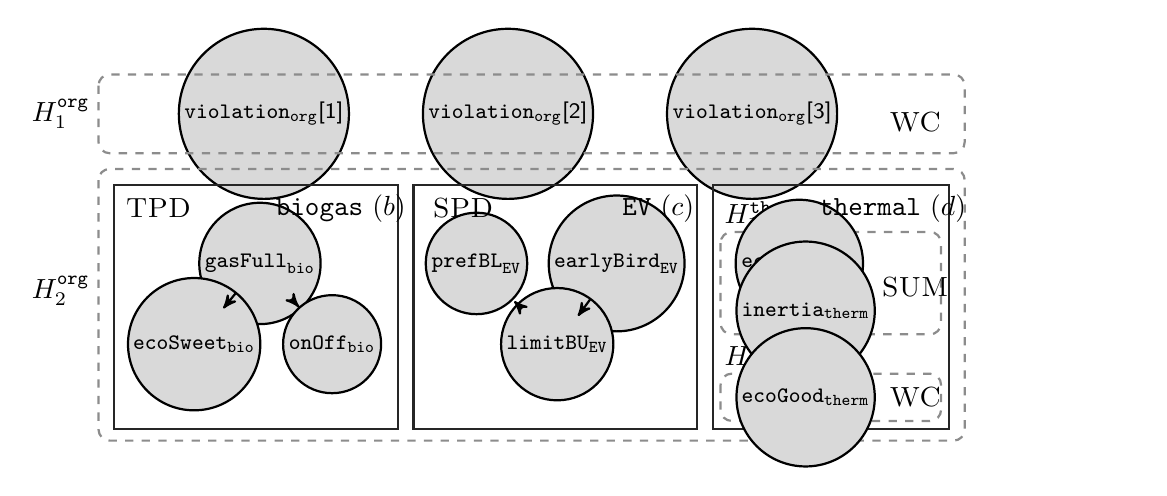
\begin{tikzpicture}[->,>=stealth',shorten >=1pt,auto,node distance=1.45cm,inner sep=1.5pt,outer sep = 0.0pt, thick] 
%\tikzstyle{every node}=[font=\tiny]
\begin{scope}[xshift=-6.0cm,yshift=-4.0cm]
\node[main node, style={font=\sffamily\footnotesize}] at (0.1,1.5) {\minMaxViolation[1]};
\node[main node, style={font=\sffamily\footnotesize}] at (3.2,1.5) {\minMaxViolation[2]};
\node[main node, style={font=\sffamily\footnotesize}] at (6.3,1.5) {\minMaxViolation[3]};

\draw [rounded corners,dashed,black!45] (-2,2) rectangle (9.0,1);
\node[text width=3cm, anchor=west, right] at (-2.9, 1.5) { \hLevelOrg{1} };
\draw [rounded corners,dashed,black!45] (-2,0.8) rectangle (9.0,-2.65);
\node[text width=4cm, anchor=west, right] at (-2.9, -0.75) { \hLevelOrg{2} };

% bio
\draw [black!85] (-1.8,0.6) rectangle (1.8,-2.5);
\node[main node, style={font=\sffamily\footnotesize}] (5) at (0.05,-0.4) {\gasFull};
\node[main node, style={font=\sffamily\footnotesize}] (6) [below left of=5,xshift=5.4] {\ecoSweet};
\node[main node, style={font=\sffamily\footnotesize}] (7) [below right of=5,xshift=-3.1] {\onOff};
%\node[main node, style={font=\sffamily\footnotesize},double] (hardConstraint) [below left of=7,xshift=-3.1,yshift=7] {$\mathsf{maxProd}$};
\node[text width=4cm, anchor=west, right] at (0.2, 0.3) { $\mathtt{\biogas}$ $(b)$ };
\node[text width=2cm, anchor=west, left] at (0.4, 0.3) { \textsc{TPD} };

% EV
\draw [black!85] (2.0,0.6) rectangle (5.6,-2.5);
\node[main node, style={font=\sffamily\footnotesize}] (3) at (2.80,-0.4) {\prefBatteryLevel};
\node[main node, style={font=\sffamily\footnotesize}] (4) at (4.58,-0.4)  {\earlyBird};
\node[main node, style={font=\sffamily\footnotesize}] (8) [below right of=3] {\limitBatteryUsage};
\node[text width=4cm, anchor=west, right] at (4.6, 0.3) { $\mathtt{\ev}$ $(c)$ };
\node[text width=2cm, anchor=west, left] at (4.3, 0.3) { \textsc{SPD} };

% thermal
\draw [black!85] (5.8,0.6) rectangle (8.8,-2.5);
\draw [rounded corners,dashed,black!45] (5.9,0) rectangle (8.7,-1.3);
\node[text width=4cm, anchor=west, right] at (5.9, 0.2) { \hLevelThermal{1} };
\draw [rounded corners,dashed,black!45] (5.9,-1.8) rectangle (8.7,-2.4);
\node[text width=4cm, anchor=west, right] at (5.9, -1.6) { \hLevelThermal{2} };
\node[main node, style={font=\ttfamily\footnotesize}] (10) at (6.9,-0.4) {\ecoOpt};
\node[main node, node distance=0.85cm, style={font=\sffamily\footnotesize}] (11) at (6.98,-1.0) {\inertia};
\node[main node, node distance=0.85cm, style={font=\sffamily\footnotesize}] (12) at (6.98,-2.1) {\ecoGood};
\node[text width=4cm, anchor=west, right] at (7.1, 0.3) { $\mathtt{\thermal}$ $(d)$ };

\node[text width=2cm, anchor=west, left] at (10, -0.7) { \textsc{SUM} };

\node[text width=2cm, anchor=west, left] at (10.1, -2.1) { \textsc{WC} };

\node[text width=2cm, anchor=west, left] at (10.1, 1.4) { \textsc{WC} };

\path[every node/.style={font=\sffamily\tiny}]
  (8) edge node [right] {} (3)
  (8) edge node [right] {} (4)
  (6) edge node [right] {} (5)
  (7) edge node [right] {} (5)
;
\end{scope}

% \begin{scope}[xshift=-0.2cm,yshift=-0.9cm]
% \node[text width=9cm,left] at (0.0, 0.0) {%
% \begin{itemize}[itemsep=2pt]
%   \item something interesting
% \end{itemize}
% };
% \end{scope}

\end{tikzpicture}
%\caption{Case study depicting individual and organizational preference specifications in context.}
\label{fig:preferencesCaseStudy}
\end{figure}
  
\begin{textblock*}{7.5cm}[1,1](\textwidth+3.8cm,\textheight-0.13cm)
\begin{itemize}
\item[] \textsc{SPD} \ldots Single-Pred.-Dom.
\item[] \textsc{TPD} \ldots Single-Pred.-Dom.
\item[] \textsc{SUM} \ldots Sum of Errors
\item[] \textsc{WC} \ldots Worst-Case Error


\end{itemize}
 \end{textblock*}


%%% Local Variables:
%%% mode: LaTeX
%%% mode: TeX-PDF
%%% mode: TeX-source-correlate
%%% TeX-master: "../quality-quantity-soft-constraints.tex"
%%% End:


Die Präferenzstruktur dieses Problems:
\vspace*{2ex}

\qquad $
  V_{\mathtt{org}_1} \ltimes (P_{\prosumer{\biogas}} \times P_{\prosumer{\ev}} \times (P_{\prosumer{\thermal}}^1 \ltimes P_{\prosumer{\thermal}}^2))
$
%
\end{frame}


\begin{frame}{Praxis I}
Third International CSP Competition (CPAI’08)
\begin{center}
\includegraphics[width=.8\textwidth]{img/cpai08.png}
\end{center}
\end{frame}

\begin{frame}{Praxis II}
Im Constraint Programming:
\begin{itemize}
\item Fokus auf \emph{klassischen} Constraint-Lösern
\item Erweiterung auf einfache Optimierung (Branch \& Bound)
\item Zielfunktion kann skalare Variable (\texttt{int} oder \texttt{float}) sein
\item { \color{isseorange} \texttt{toulbar2} ist der einzige dedizierte Weighted-CSP-Solver}
\end{itemize}

\vspace*{2ex}

In der mathematischen Programmierung:

\begin{itemize}
\item Probleme müssen gewisse Struktur aufweisen (lineare Constraints, quadratische Constraints, etc.)
\item Schlecht geeignet für beliebige Ordnungen nach denen optimiert werden soll
\end{itemize}

\vspace*{1ex} \pause 
Wir wollen aber heterogene PVS $\rightarrow$ \alert{MiniZinc}
\end{frame}


\begin{frame}{Warum MiniZinc?}
\begin{parchment}[Rationale]
\centering 
\alert{Eine Modellierungssprache -- viele Solver} 
\end{parchment}

\begin{textblock*}{2.cm}[1,1](\textwidth-.5cm,\textheight-1.03cm)

\includegraphics[width=\textwidth]{img/MiniZn_logo.jpg} 

\end{textblock*}
\emph{Reduziere Soft-Constraint-Probleme auf konventionelle Constraint-Probleme}

\begin{itemize}
\item Gecode (CP)
\item JaCoP (CP)
\item Google Optimization Tools (CP)
\item CPLEX (CP/LP/MIP)
\item G12 (CP/LP/MIP)
\item \ldots
\end{itemize}
\end{frame}


\begin{frame}[fragile]{MiniBrass}

\begin{center}

\includegraphics[width=.5\textwidth]{img/minibrass.png}

\vspace*{2ex}

\url{http://isse-augsburg.github.io/minibrass/}

\end{center}

\end{frame}

\begin{frame}[fragile]{MiniBrass: HelloWorld}
\begin{columns}[onlytextwidth,T]
    
    \begin{column}{.40\textwidth}
          
    \hSecond{Basismodell (MiniZinc)}
    \begin{lstlisting}
include "hello_o.mzn"; 
include "soft_constraints/
   pvs_gen_search.mzn"; 
% the basic, "classic" CSP 
set of int: DOM = 1..3;

var DOM: x; var DOM: y; 
var DOM: z;
% add. *hard* constraints
% e.g. constraint x < y;

solve search pvs_BAB();
\end{lstlisting}
    \end{column}
    
    \begin{column}{.55\textwidth}
  	\hFirst{Präferenzmodell (MiniBrass)} 
  	\begin{lstlisting}
PVS: cr1 = 
  new ConstraintRelationships("cr1") {
   soft-constraint c1: 'x + 1 = y';
   soft-constraint c2: 'z = y + 2';
   soft-constraint c3: 'x + y <= 3';
   
   crEdges : '[| mbr.c2, mbr.c1 | 
                  mbr.c3, mbr.c1 |]';
   useSPD: 'false' ;
}; 

solve cr1;
\end{lstlisting}

    \end{column}
  \end{columns}
  \pause
  \begin{verbatim}
Solution:  x = 1; y = 2; z = 1
Valuations:  mbr_overall_cr1 = 2..2
----------
==========
  \end{verbatim}
\end{frame}


\begin{frame} \small
\frametitle{Single-Predecessor-Dominance (SPD) Lifting}

\cemph{isWorseThan}-Relation für Mengen verletzter Constraints~\cite{Schiendorfer13}
%
\bgroup\abovedisplayskip=4pt\belowdisplayskip=12pt
\begin{gather*}
  V \uplus \{ c \}  \supset_{\mathsf{SPD}}  V 
\\
  V \uplus \{ c_{\mathrm{imp}} \}  \supset_{\mathsf{SPD}}  V \uplus \{ c_{\neg \mathrm{imp}} \}
\quad\text{if $c_{\neg \mathrm{imp}} \rightarrow c_{\mathrm{imp}}$}
\end{gather*}
\egroup

\begin{center}
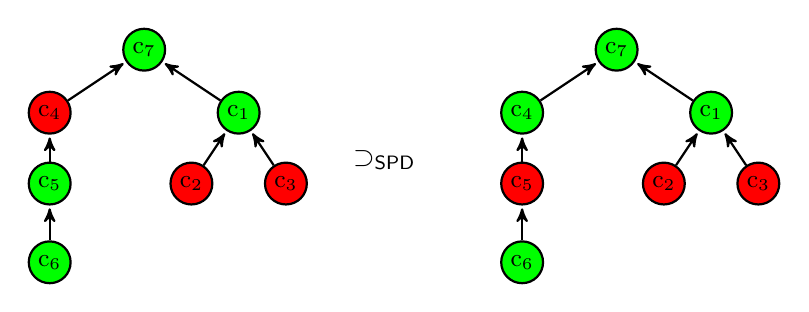
\begin{tikzpicture}[auto,
                    ->,>=stealth',shorten >=1pt,thick,
                    node distance=1cm,inner sep=2pt,
                    constraint/.style={circle,fill=black!15,draw,font=\sffamily\small}]
\begin{scope}
\node[constraint,fill=green] (1) at (0, 0)                   {$\mathrm{c}_7$};
\node[constraint,fill=red] (2) at ($ (1) + (-1.2, -0.8) $) {$\mathrm{c}_4$};  
\node[constraint,fill=green]   (3) at ($ (2) + (0.0, -0.9) $) {$\mathrm{c}_5$};  
\node[constraint,fill=green] (4) at ($ (3) + ( 0.0, -1.0) $) {$\mathrm{c}_6$};
\node[constraint,fill=green] (7) at ($ (1) + ( 1.2, -0.8) $) {$\mathrm{c}_1$};  
\node[constraint,fill=red]   (8) at ($ (7) + (-0.6, -0.9) $) {$\mathrm{c}_2$};  
\node[constraint,fill=red]   (9) at ($ (7) + ( 0.6, -0.9) $) {$\mathrm{c}_3$};  
%  
\path[every node/.style={font=\sffamily\tiny}]
  (2) edge (1)
  (7) edge (1)
  (3) edge (2)
  (4) edge (3)
  (8) edge (7)
  (9) edge (7)
  ;
\end{scope}
%
\begin{scope}[xshift=6cm]
\node[constraint,fill=green] (1) at (0, 0)                   {$\mathrm{c}_7$};
\node[constraint,fill=green]   (2) at ($ (1) + (-1.2, -0.8) $) {$\mathrm{c}_4$};  
\node[constraint,fill=red] (3) at ($ (2) + (0.0, -0.9) $) {$\mathrm{c}_5$};  
\node[constraint,fill=green] (4) at ($ (3) + ( 0.0, -1.0) $) {$\mathrm{c}_6$};  
\node[constraint,fill=green] (7) at ($ (1) + ( 1.2, -0.8) $) {$\mathrm{c}_1$};  
\node[constraint,fill=red]   (8) at ($ (7) + (-0.6, -0.9) $) {$\mathrm{c}_2$};  
\node[constraint,fill=red]   (9) at ($ (7) + ( 0.6, -0.9) $) {$\mathrm{c}_3$};  
%  
\path[every node/.style={font=\sffamily\tiny}]
  (2) edge (1)
  (7) edge (1)
  (3) edge (2)
  (4) edge (3)
  (8) edge (7)
  (9) edge (7)
  ;
\end{scope}
%
\node (R) at (3.05, -1.4) {$ \supset_{\mathsf{SPD}}$};
\end{tikzpicture}
\end{center}

\begin{itemize}
\item Bekannt als \emph{Smyth-Ordnung} (Powerdomains) \hfill \cite[Ch.~9]{amadio-curien:1998}
\item Entsteht aus \emph{freier Konstruktion} über Constraint-Relationship.\hfill \cite{knapp-schiendorfer2014ictai}
\end{itemize}

%
%\cemph{Ordnungs}relation über Zuweisungen 
%\bgroup\abovedisplayskip4pt
%\begin{equation*}
%  w \SPDord{R} v \iff \{ c \in C \mid v \not\models c \} \mathrel{({\SPDrel{R}})^{+}} \{ c \in C \mid w \not\models c \}
%\end{equation*}
%\egroup

\end{frame}

\tikzset{onslide/.code args={<#1>#2}{%
  \only<#1>{\pgfkeysalso{#2}}
}}
\tikzstyle{highlight}=[isseorange,ultra thick]
\tikzstyle{highlight2}=[CornflowerBlue,ultra thick]
\begin{frame}[fragile]{Constraint-Optimierung mit PVS}
Der partiell geordnete Bewertungsraum



\begin{figure}[!t]
\begin{center}
\begin{tikzpicture}[scale=0.77,auto]

% single PVS
\node (bot) at (0,0) {\alert{$\bot = \{c_1, c_2, c_3 \}$}};
\node (c1c2) at (-2,1) {\alert<2->{$\{c_1, c_2\}$}};
\node (c2c3) at (0,2) {$\{c_2, c_3\}$};
\node (c1c3) at (2,1) {$\{c_1, c_3\}$};

\node (c1) at (0,3) {\alert<3->{$\{c_1\}$}};
\node (c2) at (-2,4) {\alert<4->{$\{c_2\}$}};
\node (c3) at (2,4) {$\{c_3\}$};
%\node (a) at (-1,0.5) {$a$};
%\node (b) at (-1,1.5) {$b$};
%\node (c) at (1,1) {$c$};
\node (top) at (0,5) {$\top = \emptyset$};

\node[text width=2cm] (verb) at (4,0) {     };
\path[-]
(bot) edge[onslide={<2->{highlight}}] (c1c2)
      edge (c2c3)
      edge (c1c3)
(c1c2) edge (c2c3)
(c1c3) edge (c2c3)
(c1c3) edge (c1)
(c1c3) edge (c3)
(c2c3) edge (c2)
(c2c3) edge (c3)
(c1c2) edge[onslide={<3->{highlight}}] (c1)
(c1c2) edge (c2)
(c1) edge[onslide={<4->{highlight}}] (c2)
(c1) edge (c3)
(c2) edge (top)
(c1) edge (top)
(c3) edge (top)
      ;
%(a) edge (b)
%(b) edge (top)
%(bot) edge (c)
%(c) edge (top)
;

\end{tikzpicture}
\end{center}
\label{fig:nosuprema}
\end{figure}
\begin{lstlisting}
function ann: pvs_BAB() =
       repeat(
           if next() then 
                 print("Intermediate solution:") /\ print() /\
                 commit() /\ postGetBetter()
           else break endif       );
\end{lstlisting}
\begin{textblock*}{2.5cm}[1,1](\textwidth-8.8cm,\textheight-4.03cm)
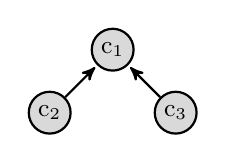
\begin{tikzpicture}[auto,
                    ->,>=stealth',shorten >=1pt,thick,
                    node distance=.7cm,inner sep=2pt,
                    constraint/.style={circle,fill=black!15,draw,font=\sffamily\small}]
\node[constraint node] (1) at (0, 0)                   {$\mathrm{c}_1$};
\node[constraint node] (2) at ($ (1) + (-0.8, -0.8) $) {$\mathrm{c}_2$};  
\node[constraint node] (3) at ($ (1) + ( 0.8, -0.8) $) {$\mathrm{c}_3$};  
%  
\path[every node/.style={font=\sffamily\tiny}]
  (2) edge (1)
  (3) edge (1)
  ;
  

\end{tikzpicture}
\begin{Verbatim}[fontsize=\small]
c1: 'x + 1 = y';
c2: 'z = y + 2';
c3: 'x + y <= 3';   
\end{Verbatim}
\end{textblock*}

\begin{textblock*}{4cm}[1,1](\textwidth+0.5cm,\textheight-3.03cm)

\onslide<2->{

{ \tt  \small
x = 1; y = 1; z = 1 \newline
Valuation = 1..2
}
}

\onslide<3->{
{ \tt  \small
----------

x = 1; y = 1; z = 3 \newline
Valuation = 1..1
}
}


\onslide<4->{
{ \tt  \small
----------

x = 1; y = 2; z = 1 \newline
Valuations = 2..2

----------

==========

}
}
\end{textblock*}
\end{frame}

\tikzset{
    process/.style={rectangle,rounded corners,draw=black, top color=isseorange!5, bottom color=isseorange!30},
    file/.style={rectangle,draw=black}
}

\begin{frame}{MiniBrass: Workflow}

\vspace*{-10ex}
\alert{Architektur}

\begin{center}
\vspace*{-10ex}
\begin{tikzpicture}[every node/.style={
anchor=base,
text depth=.5ex,
text height=2ex,
minimum height=2ex,
align=center,
circle,
minimum width=1em}]
\matrix (magic) [nodes in empty cells, ampersand replacement=\&,row sep=0.5cm,column sep=0.5cm]
{
\node[draw, file,isseorange,thick](mbr){\texttt{prefs.mbr}};  \& \& \node[draw, isseorange,thick,process](mbr2mzn){\texttt{mbr2mzn}}; \\
\node[draw, file,isseorange,thick](mbrlibs){\texttt{mbrlibs.mzn}}; \& \& \node[draw, file,isseorange,thick](compiledMzn){\emph{prefs\_o.mbr}}; \\
%    \&  \&  \node(inv){}; \&  \\
\node[draw, file](f1){\texttt{model.mzn}}; \& \& \node[draw, process](mzn2fzn){\texttt{mzn2fzn}}; \& \& \node[draw, file](output){\emph{output}};  \\
%    \&  \&  \node(inv){}; \&  \\
\node[draw, file](mod){\texttt{data.dzn}}; \& \&  \\
\& \& \node[draw, file](fzn){\texttt{compiled.fzn}}; \& \& \node[draw, process](solve){\texttt{solve}};  \\
\& \\
};

\draw[dashed,->] (f1) -- (mzn2fzn);
\draw[dashed,->] (mbr) -- (mbr2mzn);
\draw[dashed,->] (mod) -- (mzn2fzn);
\draw[dashed,->] (mbrlibs) -- (mzn2fzn);
\draw[dashed] (mbrlibs) -- (mbr);
\draw[dashed,->] (compiledMzn) -- (mzn2fzn);
\draw[dashed,->] (fzn) -- (solve);
\draw[->] (mbr2mzn) -- (compiledMzn);

\draw[->] (mzn2fzn) -- (fzn);
\draw[->] (solve) -- (output);
%\draw[dashed] (globals) -- (inv);
\end{tikzpicture}
\end{center}
\vspace*{-25ex}

\end{frame}

\begin{frame}

\end{frame}

\begin{frame}{Evaluationsergebnisse}

\end{frame}

\begin{frame}{Kooperationen}
\begin{itemize}
\item[] \alert{Konzepte, Sprachdesign MiniBrass}
\begin{itemize}
\item[-] AS, Alexander Knapp, Gerrit Anders, Oliver Kosak
\end{itemize}
\item[] \alert{Anwendungen, Multiagenten-Einsatz}
\begin{itemize}
\item[-] Alexander Schubert (MSc-Thesis: Einsatz von Voting-Verfahren), Markus Tolls (MSc-Thesis: Formalisierung von Task-Allocation-Problemen)
\end{itemize}
\end{itemize}
\end{frame}

\begin{frame}{Outreach}
\begin{itemize}
\item Vortrag Helmholtz-Zentrum München
\item Vortrag FH Hagenberg
\item Tutorial @ SASO 2016
\end{itemize}
\end{frame}



\begin{frame}[allowframebreaks]
        \frametitle{References}
        \bibliographystyle{apalike}
        \bibliography{../common}
\end{frame}


\end{document}

